\documentclass[journal]{IEEEtran}

% *** CITATION PACKAGES ***
\usepackage{cite}

% *** GRAPHICS RELATED PACKAGES ***
%
\ifCLASSINFOpdf
\usepackage[pdftex]{graphicx}
  % declare the path(s) where your graphic files are
  % \graphicspath{{../pdf/}{../jpeg/}}
  % and their extensions so you won't have to specify these with
  % every instance of \includegraphics
  % \DeclareGraphicsExtensions{.pdf,.jpeg,.png}
\else
  % or other class option (dvipsone, dvipdf, if not using dvips). graphicx
  % will default to the driver specified in the system graphics.cfg if no
  % driver is specified.
  % \usepackage[dvips]{graphicx}
  % declare the path(s) where your graphic files are
  % \graphicspath{{../eps/}}
  % and their extensions so you won't have to specify these with
  % every instance of \includegraphics
  % \DeclareGraphicsExtensions{.eps}
\fi
% graphicx was written by David Carlisle and Sebastian Rahtz. It is
% required if you want graphics, photos, etc. graphicx.sty is already
% installed on most LaTeX systems. The latest version and documentation
% can be obtained at: 
% http://www.ctan.org/pkg/graphicx
% Another good source of documentation is "Using Imported Graphics in
% LaTeX2e" by Keith Reckdahl which can be found at:
% http://www.ctan.org/pkg/epslatex
%
% latex, and pdflatex in dvi mode, support graphics in encapsulated
% postscript (.eps) format. pdflatex in pdf mode supports graphics
% in .pdf, .jpeg, .png and .mps (metapost) formats. Users should ensure
% that all non-photo figures use a vector format (.eps, .pdf, .mps) and
% not a bitmapped formats (.jpeg, .png). The IEEE frowns on bitmapped formats
% which can result in "jaggedy"/blurry rendering of lines and letters as
% well as large increases in file sizes.
%
% You can find documentation about the pdfTeX application at:
% http://www.tug.org/applications/pdftex






% *** PDF, URL AND HYPERLINK PACKAGES ***
%
%\usepackage{url}
% url.sty was written by Donald Arseneau. It provides better support for
% handling and breaking URLs. url.sty is already installed on most LaTeX
% systems. The latest version and documentation can be obtained at:
% http://www.ctan.org/pkg/url
% Basically, \url{my_url_here}.


% correct bad hyphenation here
\hyphenation{op-tical net-works semi-conduc-tor}


\begin{document}
%
% paper title
% Titles are generally capitalized except for words such as a, an, and, as,
% at, but, by, for, in, nor, of, on, or, the, to and up, which are usually
% not capitalized unless they are the first or last word of the title.
% Linebreaks \\ can be used within to get better formatting as desired.
% Do not put math or special symbols in the title.
\title{Diseño de Experimentos para la Comparación de Modelos de Clasificación de Textos en Noticias Reales y Falsas}


\author{Álvaro Salgado López}

% note the % following the last \IEEEmembership and also \thanks - 
% these prevent an unwanted space from occurring between the last author name
% and the end of the author line. i.e., if you had this:
% 
% \author{....lastname \thanks{...} \thanks{...} }
%                     ^------------^------------^----Do not want these spaces!
%
% a space would be appended to the last name and could cause every name on that
% line to be shifted left slightly. This is one of those "LaTeX things". For
% instance, "\textbf{A} \textbf{B}" will typeset as "A B" not "AB". To get
% "AB" then you have to do: "\textbf{A}\textbf{B}"
% \thanks is no different in this regard, so shield the last } of each \thanks
% that ends a line with a % and do not let a space in before the next \thanks.
% Spaces after \IEEEmembership other than the last one are OK (and needed) as
% you are supposed to have spaces between the names. For what it is worth,
% this is a minor point as most people would not even notice if the said evil
% space somehow managed to creep in.








% If you want to put a publisher's ID mark on the page you can do it like
% this:
%\IEEEpubid{0000--0000/00\$00.00~\copyright~2015 IEEE}
% Remember, if you use this you must call \IEEEpubidadjcol in the second
% column for its text to clear the IEEEpubid mark.



% use for special paper notices
%\IEEEspecialpapernotice{(Invited Paper)}


\markboth{Procesamiento Y Clasificación de Datos, 30 Enero 2025}{}

% make the title area
\maketitle



%\IEEEpeerreviewmaketitle



\section{Introducción}
% The very first letter is a 2 line initial drop letter followed
% by the rest of the first word in caps.
% 
% form to use if the first word consists of a single letter:
% \IEEEPARstart{A}{demo} file is ....
% 
% form to use if you need the single drop letter followed by
% normal text (unknown if ever used by the IEEE):
% \IEEEPARstart{A}{}demo file is ....
% 
% Some journals put the first two words in caps:
% \IEEEPARstart{T}{his demo} file is ....
% 
% Here we have the typical use of a "T" for an initial drop letter
% and "HIS" in caps to complete the first word.
\IEEEPARstart
{L}{a} proliferación de noticias falsas en medios digitales ha generado la necesidad de desarrollar métodos automáticos para su detección. Dentro del procesamiento de lenguaje natural (NLP), el aprendizaje automático ofrece herramientas eficientes para la clasificación de textos, permitiendo diferenciar entre información veraz y engañosa con alta precisión.

Este estudio tiene como objetivo comparar distintos modelos de clasificación de texto y evaluar el impacto de sus hiperparámetros en el desempeño de la detección de noticias falsas. Para ello, se utilizó el conjunto de datos “Fake and Real News” de Kaggle, compuesto por noticias etiquetadas como reales o falsas.

En el diseño del experimento, se implementaron varios algoritmos de clasificación, incluyendo Naive Bayes, Regresión Logística y Máquinas de Vectores de Soporte (SVM). Para optimizar los hiperparámetros se empleó GridSearchCV, un método de búsqueda exhaustiva basado en validación cruzada, lo que permitió identificar las configuraciones óptimas para cada clasificador.

El desempeño de los modelos se evaluó utilizando métricas como precisión, recall, F1-score y accuracy, además de analizar la matriz de confusión para interpretar los errores de clasificación. Los resultados de este análisis permitirán determinar qué modelo y combinación de hiperparámetros ofrece la mejor solución para la detección automática de noticias falsas.
% You must have at least 2 lines in the paragraph with the drop letter
% (should never be an issue)

\section{Metodología}
En esta sección se describe el procedimiento seguido para la clasificación de noticias falsas y reales, desde la preparación de los datos hasta la evaluación de los modelos empleados.

\subsection{Preprocesamiento de los Datos}

El conjunto de datos utilizado proviene de la plataforma Kaggle y contiene noticias etiquetadas como reales o falsas. Antes de aplicar los modelos de clasificación, se realizó un preprocesamiento del texto con el objetivo de mejorar la calidad de los datos y eliminar elementos que pudieran introducir ruido en el análisis.

Las etapas del preprocesamiento fueron las siguientes:
\begin{itemize}
    \item Normalización del texto: Conversión de todos los caracteres a minúsculas para evitar discrepancias entre palabras con diferentes capitalizaciones.
    \item Eliminación de caracteres especiales: Se eliminaron signos de puntuación y otros símbolos no alfabéticos.
    \item Construcción del corpus de texto: Se concatenaron los títulos y el contenido de las noticias en una única columna, con el propósito de preservar la información de ambas fuentes.
\end{itemize}

Una vez limpiado el texto, se aplicó una técnica de representación numérica de los datos. Para ello, se utilizó la técnica TF-IDF (Term Frequency-Inverse Document Frequency), la cual asigna pesos a cada palabra en función de su frecuencia en los documentos y en el conjunto total de datos. En este caso, se estableció un límite de 5000 características y se eliminaron las palabras vacías en inglés para reducir la dimensionalidad del espacio de características.

\subsection{División del Conjunto de Datos}

Para evaluar el desempeño de los modelos, se realizó una partición del conjunto de datos en 80 \% para entrenamiento y 20 \% para prueba. Se utilizó una estrategia de división estratificada para garantizar que la distribución de clases en cada subconjunto reflejara la del conjunto original.

\subsection{Modelos de Clasificación}

Se implementaron y compararon diversos modelos de clasificación con el objetivo de determinar cuál proporciona el mejor desempeño en la tarea de detección de noticias falsas. Los modelos evaluados fueron los siguientes:
\begin{itemize}
    \item Naive Bayes Multinomial
    \item Regresión Logística
    \item Máquinas de Soporte Vectorial (SVM)
\end{itemize}

Cada uno de estos modelos fue entrenado utilizando el conjunto de datos preprocesado y vectorizado con TF-IDF.

\subsection{Ajuste de Hiperparámetros}

En particular, para la Regresión Logística, se realizó una búsqueda aleatoria con los siguientes hiperparámetros:
\begin{itemize}
    \item C: Parámetro de regularización con valores extraídos de una distribución uniforme en el intervalo [0.1, 10].
    \item Penalty: Penalización L1 y L2 para regularización.
    \item Solver: Se utilizó liblinear para permitir el uso de la penalización L1.
    \item Validación cruzada: Se empleó un esquema de validación de 5 particiones (5-fold cross-validation).
\end{itemize}
5. Evaluación de los Modelos

Los modelos fueron evaluados con base en las siguientes métricas:
\begin{itemize}
    \item Precisión (Accuracy): Proporción de predicciones correctas en el conjunto de prueba.
    \item Matriz de confusión: Representación de los errores de clasificación en términos de verdaderos positivos, falsos positivos, verdaderos negativos y falsos negativos.
    \item Puntajes de Precision, Recall y F1-score: Medidas de desempeño para evaluar la capacidad del modelo de distinguir entre noticias falsas y reales.
    \item Análisis de palabras más importantes: Se identificaron las palabras más relevantes para la clasificación de noticias falsas y reales a través del análisis de los pesos asignados por el vectorizador TF-IDF.
    \item Conteo de palabras: Se realizaron análisis de frecuencia para comparar las palabras más comunes en noticias falsas y reales. A partir de estos conteos, se generaron representaciones visuales mediante nubes de palabras y gráficos de barras para facilitar la interpretación.
\end{itemize}
	
\section{Resultados}
En este estudio se compararon tres modelos de clasificación de texto para detectar noticias falsas, utilizando el conjunto de datos de noticias falsas y reales disponible en Kaggle. Los modelos evaluados fueron Naive Bayes, Regresión Logística y Support Vector Machine (SVM). Además, se utilizó la técnica de RandomizedSearchCV para optimizar los hiperparámetros del modelo de Regresión Logística.

\subsection{Desempeño de los Modelos}

Los tres modelos fueron evaluados utilizando las métricas de precisión (accuracy), recall, f1-score y la matriz de confusión. A continuación, en la Tabla \ref{table:resultados_modelos} se presentan los resultados de cada modelo:

\begin{table}[ht]
\centering
\begin{tabular}{|c|c|c|c|}
\hline
\textbf{Modelo} & \textbf{Precisión} & \textbf{Recall} & \textbf{F1-score} \\
\hline
\textbf{Naive Bayes} & 0.93 & 0.93 & 0.93 \\
\textbf{Noticias Reales (0)} & 0.93 & 0.93 & 0.93 \\
\textbf{Noticias Falsas (1)} & 0.94 & 0.94 & 0.94 \\
\hline
\textbf{Regresión Logística} & 0.99 & 0.99 & 0.99 \\
\textbf{Noticias Reales (0)} & 0.98 & 0.99 & 0.99 \\
\textbf{Noticias Falsas (1)} & 0.99 & 0.98 & 0.99 \\
\hline
\textbf{SVM} & 0.99 & 0.99 & 0.99 \\
\textbf{Noticias Reales (0)} & 0.99 & 1.00 & 0.99 \\
\textbf{Noticias Falsas (1)} & 1.00 & 0.99 & 0.99 \\
\hline
\end{tabular}
\caption{Resultados de precisión, recall y f1-score de los modelos evaluados.}
\label{table:resultados_modelos}
\end{table}

Naive Bayes alcanzó una precisión de 0.93 en ambas clases (noticias verdaderas y falsas), mostrando una buena capacidad para manejar la dispersión de las clases en el conjunto de datos. Este modelo es conocido por ser eficiente y rápido, especialmente en tareas de clasificación de texto, y su rendimiento en este caso no fue la excepción.

Por otro lado, Regresión Logística alcanzó una precisión significativamente más alta de 0.99, tanto en noticias verdaderas como falsas. Este modelo mostró una alta capacidad de generalización y una excelente distinción entre las clases, lo que lo posicionó como una opción muy sólida para la tarea de clasificación de noticias.

Máquinas de Vectores de Soporte (SVM) también mostró un desempeño sobresaliente con una precisión de 0.99, sin embargo, se observó que el tiempo de entrenamiento fue considerablemente mayor en comparación con los otros modelos. Este comportamiento se debe a la complejidad inherente al entrenamiento de SVM, especialmente cuando se trabaja con grandes volúmenes de datos y una cantidad significativa de características, como es el caso del conjunto de datos utilizado en este estudio.

Por esta razón, aunque SVM mostró un rendimiento muy cercano al de la regresión logística, se optó por utilizar Regresión Logística para la optimización de los hiperparámetros, debido a su menor tiempo de entrenamiento sin sacrificar el desempeño. La optimización de los hiperparámetros de la regresión logística se realizó mediante el uso de RandomizedSearchCV, lo que permitió encontrar los mejores valores de los parámetros clave (C, penalty, solver) y mejorar aún más su precisión.

La validación cruzada utilizada durante la optimización mostró que el modelo de regresión logística con los hiperparámetros optimizados alcanzó una precisión en el conjunto de prueba de 0.9959, lo que confirma que este modelo no solo es eficiente en cuanto a tiempo, sino también altamente preciso.

\subsection{Relevancia de las palabras}
Las palabras más frecuentes en las noticias falsas y reales, según el análisis de TF-IDF, revelan patrones significativos en el uso del lenguaje en ambas categorías.

En las noticias falsas, los términos más frecuentes incluyen nombres y temas políticos asociados con figuras prominentes, como “america”, “trump”, “clinton”, “obama”, “hillary”, y “donald”. Estos términos reflejan una tendencia a centrarse en figuras y eventos políticos específicos, particularmente relacionados con las campañas electorales. La presencia de palabras como “media”, “news”, “video”, “time”, y “state” también sugiere un enfoque hacia los temas de actualidad, los medios de comunicación y la cobertura informativa.

En contraste, las noticias reales muestran una distribución de palabras más asociada con temas generales de política y gobernanza, como “campaign”, “election”, “government”, “party”, y “republican”. Las noticias reales tienden a enfocarse en términos más formales y específicos relacionados con el gobierno y las elecciones, con términos recurrentes como “president”, “states”, “washington”, y “united”.

En la Fig \ref{fig:count} se aprecia el conteo de las palabras para cada categoría noticias

\begin{figure}
    \centering
    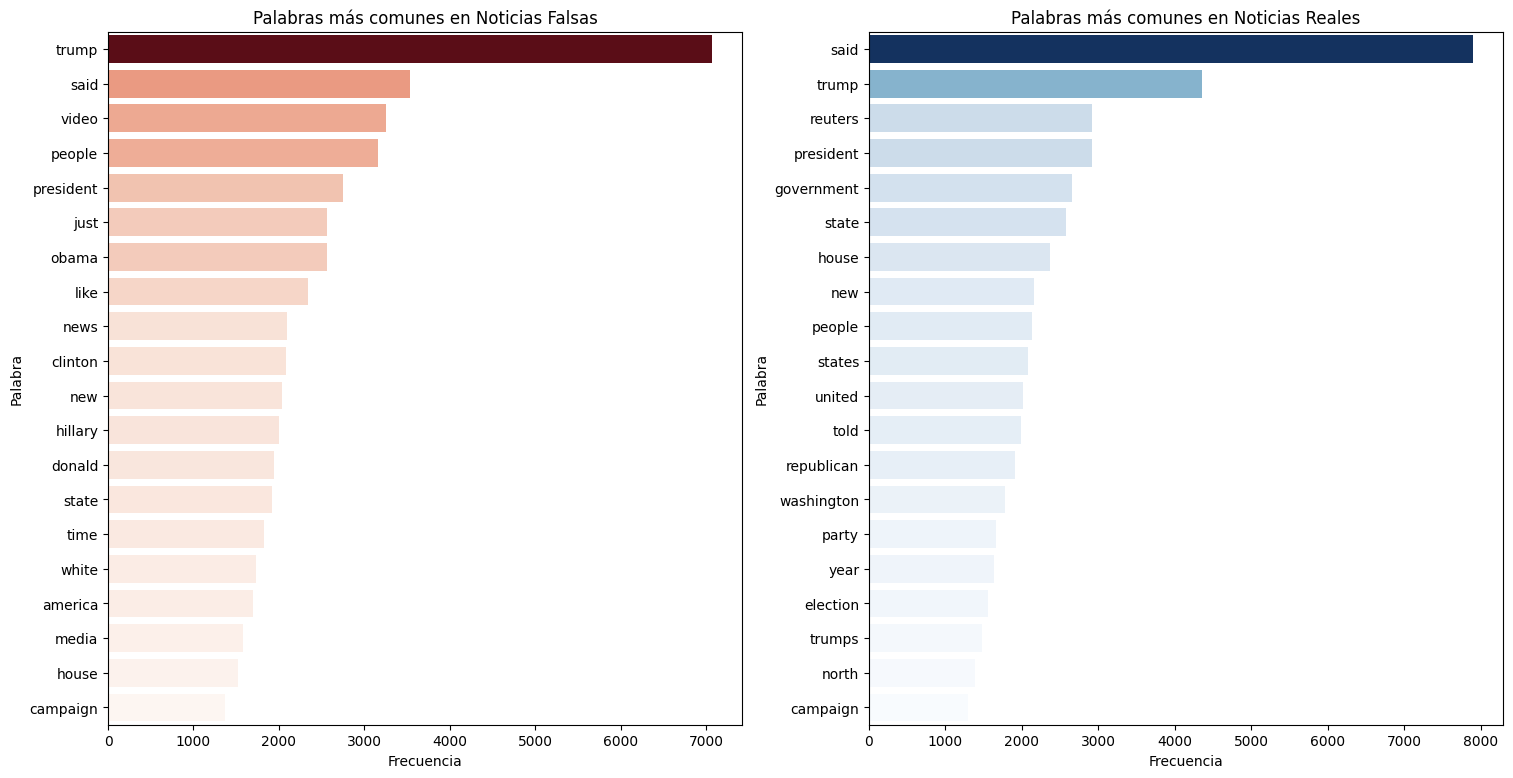
\includegraphics[width=0.8\linewidth]{Figs/word_count.png}
    \caption{Conteo de palabras}
    \label{fig:count}
\end{figure}

Estos resultados evidencian la diferencia en el enfoque temático entre las noticias reales y las falsas. Las noticias falsas tienden a estar más centradas en nombres específicos y temas relacionados con figuras políticas, mientras que las noticias reales se enfocan más en procesos electorales y políticos, con un vocabulario más institucional y generalizado.

Este análisis permite visualizar las diferencias clave entre las dos categorías de noticias, ofreciendo una base sólida para la clasificación y la detección de noticias falsas a través del modelo entrenado.

\section{Conclusión}
El objetivo principal de este estudio fue realizar un diseño de experimentos para comparar diferentes modelos de clasificación y sus hiperparámetros en relación con la tarea de clasificación de noticias reales y falsas. Se utilizaron tres modelos principales: Naive Bayes, Regresión Logística y SVM, con el propósito de identificar cuál de ellos se adapta mejor a los datos y ofrece un desempeño superior.

Los resultados mostraron que todos los modelos tuvieron un desempeño sobresaliente, con SVM y Regresión Logística alcanzando una precisión cercana al 99\%. Sin embargo, el uso de técnicas de optimización, como el RandomizedSearchCV para la Regresión Logística, permitió mejorar la precisión del modelo y reducir los tiempos de entrenamiento, lo que hace que este modelo sea la opción más eficiente en términos de recursos computacionales. La optimización de los hiperparámetros a través de esta técnica contribuyó a una precisión final de 99.6%, superando al modelo SVM, que presentó tiempos de entrenamiento más largos.

A través del análisis de las palabras más frecuentes en las noticias reales y falsas utilizando el método TF-IDF, se observó una clara diferencia en los términos utilizados en cada categoría, lo cual validó que las características textuales son clave para la clasificación. Las noticias falsas tendieron a tener un vocabulario más centrado en nombres de figuras políticas y controversias, mientras que las noticias reales mostraron un enfoque más institucional y político.

Finalmente, la comparación de los modelos mediante métricas como precisión, recall y F1-score, junto con la validación cruzada, demostró que la Regresión Logística optimizada fue la que mejor desempeño tuvo, lo que confirma que la selección adecuada de hiperparámetros es crucial para mejorar el rendimiento de los modelos de clasificación de texto.

Este análisis resalta la importancia de aplicar un diseño de experimentos adecuado en tareas de clasificación, permitiendo la evaluación precisa y eficiente de los modelos y la mejora de su rendimiento a través de la optimización de parámetros.
% Can use something like this to put references on a page
% by themselves when using endfloat and the captionsoff option.
\ifCLASSOPTIONcaptionsoff
  \newpage
\fi



% trigger a \newpage just before the given reference
% number - used to balance the columns on the last page
% adjust value as needed - may need to be readjusted if
% the document is modified later
%\IEEEtriggeratref{8}
% The "triggered" command can be changed if desired:
%\IEEEtriggercmd{\enlargethispage{-5in}}

% references section

% can use a bibliography generated by BibTeX as a .bbl file
% BibTeX documentation can be easily obtained at:
% http://mirror.ctan.org/biblio/bibtex/contrib/doc/
% The IEEEtran BibTeX style support page is at:
% http://www.michaelshell.org/tex/ieeetran/bibtex/
%\bibliographystyle{IEEEtran}
% argument is your BibTeX string definitions and bibliography database(s)
%\bibliography{IEEEabrv,../bib/paper}
%
% <OR> manually copy in the resultant .bbl file
% set second argument of \begin to the number of references
% (used to reserve space for the reference number labels box)

%\bibliographystyle{IEEEtran} % Estilo de citas de IEEE
%\bibliography{referencias} % Nombre de tu archivo .bib


\end{document}


